% Contributors: Last semester's scribes...
% Contributors: Greg Kocher, Wenbo Gao, Sahil Manocha
\section{Embedding into $l_\infty^d$} 
%sectioning used above is autocapitalizing 
%and confusing little d with big D in header on every odd pg...
Reminder: $||u-v||_{l_\infty^d}=\max_{1\leq i \leq d} |u_i-v_i|$\\


\begin{theorem}[Fr\'echet]
Any $n$-point metric space $(\mathbf{X}, \rho)$ with $|\mathbf{X}|=n$
can be isometrically embedded into $l_\infty^d (d=n)$.  
\end{theorem}
\begin{proof}
Let $x \in \mathbf{X}$, consider the function 
\[
f(x)=
\begin{bmatrix}
    \rho (x,x_1)\\
    \rho (x,x_2)\\
    ...\\
    \rho (x,x_n)
\end{bmatrix}
\]
\textbf{Claim 1}: $f$ is a contraction. That is, $\forall u,v \in
\mathbf{X}$, $||f(u)-f(v)||_{l_\infty^d} \leq \rho (u,v)$.\\ 
Observation: Because $\rho$ is a metric, by the triangle
inequality, 
\[
\forall x_i \in \mathbf{X},\ \rho (u,x_i) - \rho (v,x_i) \leq \rho
(u,v) 
\]
Since the triangle inequality holds for any $u$ and $v$,
including some pair of $u$ and $v$ which maximizes the left
side, it follows that 
\[
\max_{u,v} | \rho (u,x_i) - \rho (v,x_i)| \leq \rho (u,v),\]
or rewriting this directly in terms of the metric induced by
the $l_\infty$-norm,
\[
||f(u)-f(v)||_{l_\infty^d} \leq \rho (u,v)
\]
\\
\textbf{Claim 2}: $\forall u,v \in X, \exists i$ such that $\rho (u,v) 
\leq (f(u)-f(v))_{i}$.\\
Observation: The expression above for $f(x)$ applies to any $x$,
including $x=v$ and $x=u$ for the particular points
$u,v$ under 
consideration.
Thus we have
\[
f(u)=
\begin{bmatrix}
\rho (u,x_1)\\
...\\
\rho (u,v)\\
\rho (u,x_n)
\end{bmatrix}
\]
and
\[
f(v)=
\begin{bmatrix}
\rho (v,x_1)\\
...\\
\rho (v,v)\\
\rho (v,x_n)
\end{bmatrix}
\]
Taking the $i^{th}$ row (corresponding to point $v$) 
of the vectors $f(u)$ and $f(v)$,
we get
\[
[f(u)-f(v)]_{i} = f(u)_{i}-f(v)_{i} = \rho (u,v) - \rho (v,v)
= \rho (u,v).
\]
But since we are using the metric induced by the 
$l_\infty$-norm, we end up taking a max over all elements of
the vector $[f(u)-f(v)]$, so $||f(u)-f(v)||_{l_\infty}$
is at least as big as it's $i^{th}$ element
$\rho (u,v)$, so we can write
$\rho (u,v) \leq ||f(u)-f(v)||_{l_\infty^d}$.

We can bound the $l_\infty$-norm metric
on both sides by combining Claim 1 and Claim 2. Claim 1 gives an 
upper bound (right inequality below), and Claim 2 gives a lower bound
(left inequality below):
\[
\rho (u,v) \leq ||f(u)-f(v)||_{l_\infty^d} \leq \rho (u,v)
\]\\
Since the upper and lower bounds are the same, they are equal 
to the middle quantity, so
\[
||f(u)-f(v)||_{l_\infty^d} = \rho (u,v),
\]
so $D=r=1$, so $f$ is an isometric embedding of the
$n$-point metric space $(\mathbf{X}, \rho)$ 
into $l_\infty^d (d=n)$.
\end{proof}

This is why $l_\infty$ is considered a universal embedding space. 
In general, of the common $l_p$-norms, 
$l_\infty$ is the easiest to embed into, $l_1$ is hard, and $l_2$
is the hardest. Conceptually, we can represent this
relationship between $l_p$-norm and embedding difficulty
with this very approximate sketch, where the 
difficulty of embedding is e.g. the lowest distortion 
achievable for a given metric.\\

\begin{figure}[h!]
\begin{center}
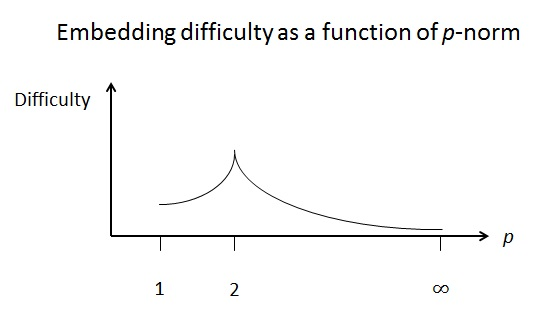
\includegraphics[width=0.5\textwidth]{chapter_5/files/embedding_difficulty.jpg}
\caption{Conceptual idea of embedding difficulty as
a function of $l_p$-norm.}
\end{center}
\end{figure}



\textbf{Question}: Can we do any better than
$d=n$ from Fr\'echet's Embedding?

\textbf{Answer}: We can at least improve to $d=n-1$. Claim 2 above 
hints at this.
When considering the $i^{th}$ component, we looked at 
the coordinate corresponding to $v$ but could also have looked at the
coordinate corresponding to $u$, and this redundancy suggests our mapping $f$
is not as frugal as possible with coordinates. In fact, we can get an
isometric embedding with $l_\infty^{n-1}$.\\

\textbf{Question}: Can we do significantly better (e.g. $d=o(n)$) than
$d=n$ from Fr\'echet's Embedding?

\textbf{Answer}: The Incompressibility Theorem says no, unless we
allow distortion.

\begin{theorem}[Incompressibility of general metric spaces]
If $\mathbf{Z}$ is a normed space that $D$-embeds all $n$-points
metric space, then,\\ dim$(\mathbf{Z})=\Omega (n)$ for $D<3$.\\ 
dim$(\mathbf{Z})=\Omega (n^{1/2})$ for $D<5$.\\
dim$(\mathbf{Z})=\Omega (n^{1/3})$ for $D<7$.
\end{theorem}
Observations: The trend of smaller embedded dimension with 
increased distortion makes sense: more compression requires 
more distortion. Also, notice that the distortion values $D$
change in discrete steps rather than varying continuously. \\
\\
\textbf{Proof Sketch}\\
Consider a collection of $n$-vertex graphs that have a
girth (length of shortest cycle) of size 
at least $l$. In particular, we'll want to use 
high girth graphs.
The edge incidences are not important for this argument.
Try to embed all such graphs into a normed space $\mathbf{Z}$ with 
dim$(\mathbf{Z})=o(n)$
 without incurring any distortion. 
Use a volume argument, saying that each
graph occupies some part of the space, and by embedding all
the graphs in that space, you eventually run out of room and
would need more volume. Therefore, from this volume argument,
it is not possible to embed any arbitrary n-point metric space
into such a $Z$ with dim$(\mathbf{Z})=o(n)$. 
Therefore, we must have dim$(\mathbf{Z})= \Omega (n)$.
However, if we are willing to incur some distortion, we 
can do better. \\
\\
\textbf{Open Question}: How many $n$-vertex graphs exist 
with a given girth? There are inexact upper and lower
bounds, but if we could enumerate them exactly, we could
improve our incompressibility bounds. \\
\\

\begin{theorem}[Construction is due to Bourgain]
Let $D=3$ and $(\mathbf{X},\rho)$ be a $n$-point metric space. Then
there exists a $D$-embedding of $\mathbf{X}$
into $l_\infty^d$ with
$d=\ceil{48\sqrt{n}\ln n}=O(\sqrt{n}\ln n)$.
\end{theorem}
\textbf{Proof Sketch}\\
Since we are treating the case of distortion $D=3$, we want 
to have a coordinate such that 
$\frac{1}{3}\rho(u,v) \leq [f(u)-f(v)]_i
\leq \rho(u,v)$. Using ideas from
Fr\'echet's Theorem, we'll create a mapping

\[
f(u)=
\begin{bmatrix}
    \rho (u,A_1)\\
    \rho (u,A_2)\\
    ...\\
    \rho (u,A_d)
\end{bmatrix}
\]
where $A_i \subset \mathbf{X}$ and $\rho (u,A) = \min_{x \in A} 
\rho(u,x)$. We'll show that we can make $f$ so that
we get the desired factor of $3$, and use a probabilistic 
argument to say that this mapping $f$ exists.\\

\begin{figure}[h!]
\begin{center}
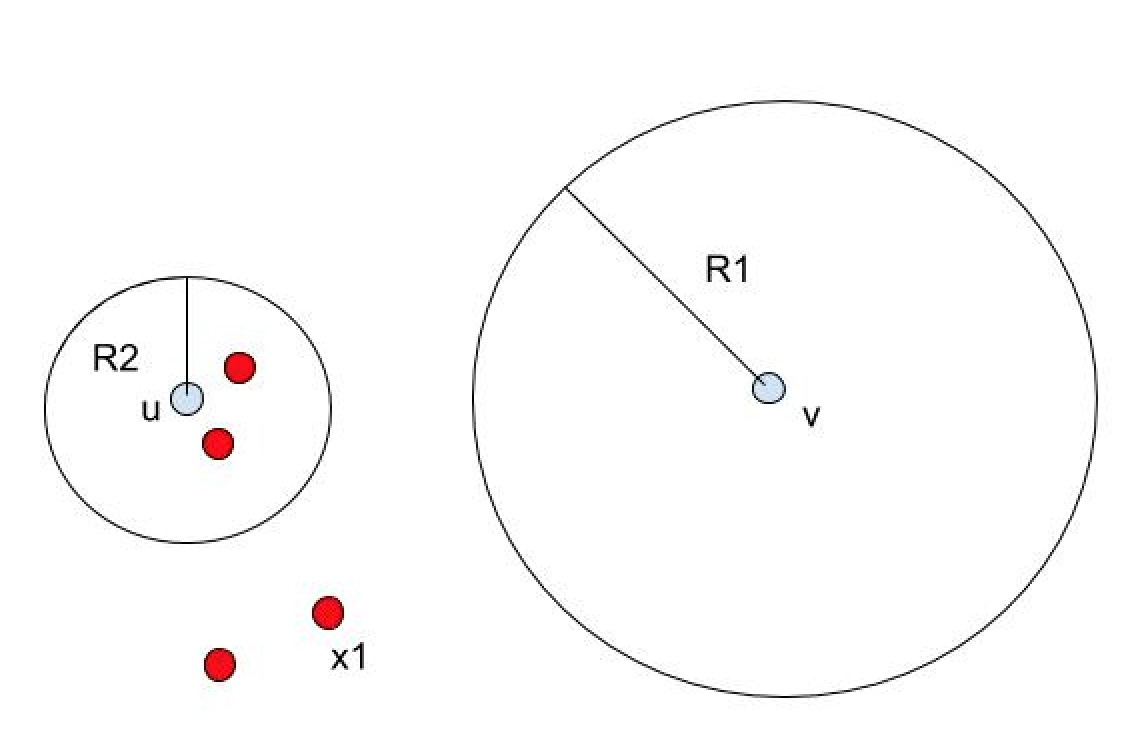
\includegraphics[width=0.5\textwidth]{chapter_5/files/construction.jpg}
\caption{An illustration of the construction in the proof}
\end{center}
\end{figure}

\textbf{Idea}: In Fr\'echet's Theorem, we used a map $f$
that considered pairwise distances between points. Every
coordinate of $f(x)$ was the distance from $x$ to some
$x'$. We can extend this idea and look at the distance from
point $x$ to various sets of points instead of distances 
to other individual points. 
This will be more economical than just one coordinate
per pair of distances: ideally each coordinate will encode
more information so that we can use fewer coordinates and 
achieve a lower dimension 
embedding, while incurring some specified distortion.\\

\textbf{Formal Proof}
\begin{proof}
  Let $m=\ceil{24 \sqrt{n} \ln n}$. For $i=1, ..., m$:
  \begin{enumerate}
  \item[1.] Starting from the empty set, construct the set $A_i$.
  For every 
  $x \in \mathbf{X}$, include it in the set $A_i$ with probability
    $\min (\frac{1}{2}, \frac{1}{\sqrt{n}})$, where the 
    decision for each $x$ is made independently.
  \item[2.] Starting from the empty set,
  construct the set $\bar{A}_i$. 
  For every 
  $x \in \mathbf{X}$, include it in the set $\bar{A}_i$ 
  with probability
    $\min (\frac{1}{2}, \frac{1}{n})$, where the 
    decision for each $x$ is made independently.\\  
  \end{enumerate}
Note that $\bar{A}_i$ is constructed independently of $A_i$, so 
    the two sets can have arbitrary overlap in points, i.e. 
    the overbar does not denote
    complementary sets, so a point $x$ may be in both 
    $A_i$ and $\bar{A}_i$. Furthermore, each pair of sets
    subscripted by $i$ is selected independently of the pair
    of sets indexed by $j$, so again the set memberships
    of the points are arbitrary.
    
We'll use these sets to define the coordinates of the 
mapping $f$. In total there will be $2m$ coordinates defined as:

\[
\forall x \in \mathbf{X}, f(x)=
\begin{bmatrix}
    \rho (x,A_1)\\
    \rho (x,A_2)\\
    ...\\
    \rho (x,A_m)\\
    \rho (x,\bar{A}_1)\\
    \rho (x,\bar{A}_2)\\
    ...\\
    \rho (x,\bar{A}_m)\\
\end{bmatrix}
\]
\textbf{Claim}: Pick any $u,v \in \mathbf{X},u\neq v$ and pick $i$.
Then either \\
$|\rho (u,A_i)-\rho (v,A_i)| \geq \frac{1}{3} \rho (u,v)$ or \\
$|\rho (u,\bar{A_i})-\rho (v,\bar{A_i})|\geq \frac{1}{3} \rho (u,v)$,\\
with
probability $\geq \frac{1}{12\sqrt{n}}$ (over the choices of $A_i$ and
$\bar{A_i}$). 

\begin{figure}[h!]
\begin{center}
\caption{An illustration of the three balls}
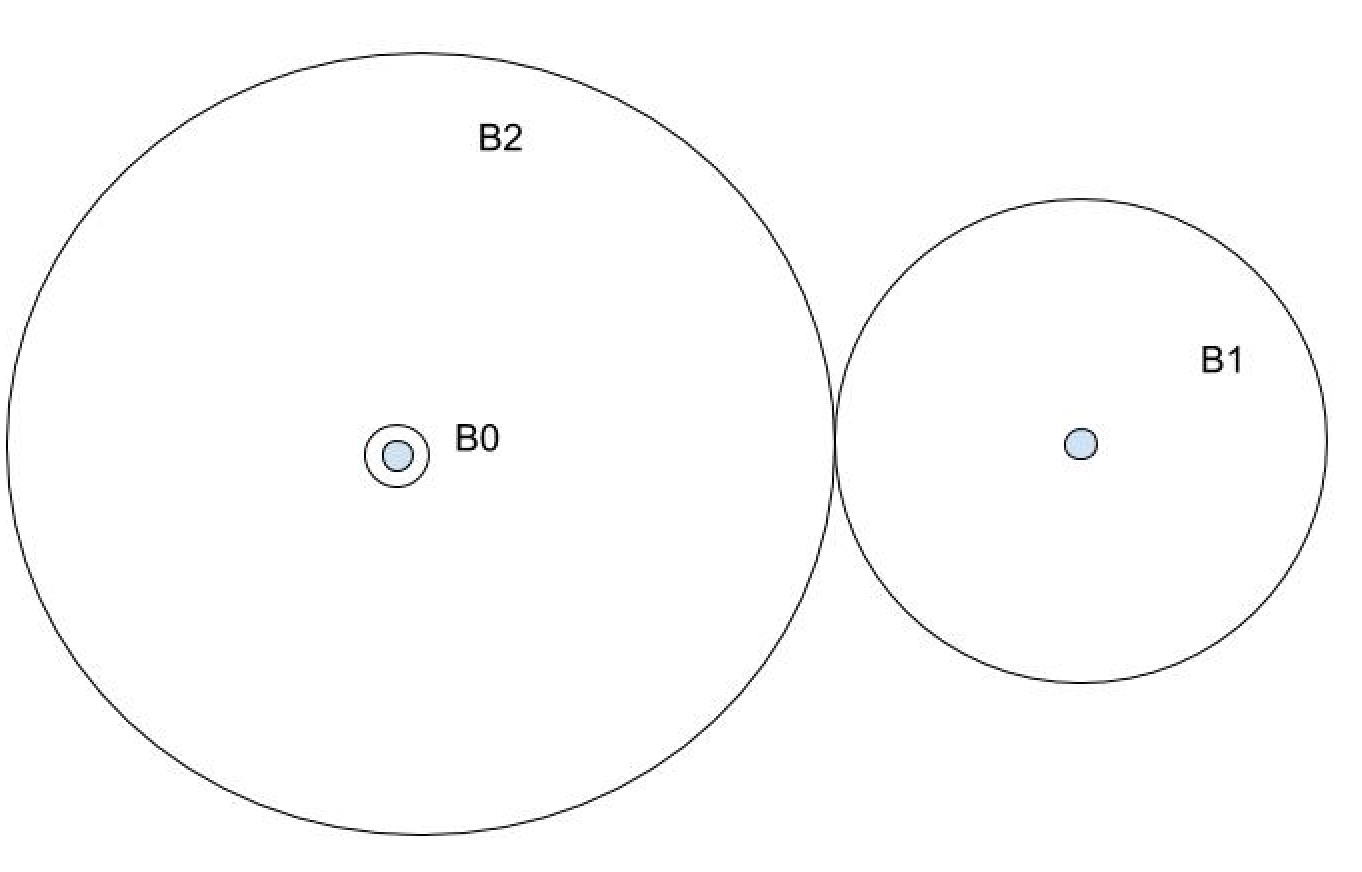
\includegraphics[width=0.5\textwidth]{chapter_5/files/three_balls.jpg}
\end{center}
\end{figure}
\textbf{Idea}: If the first condition holds, then the $i^{th}$ 
coordinate
of $[f(u)-f(v)]$, i.e. 
$[f(u)-f(v)]_i$,
is $\geq \frac{1}{3} \rho (u,v)$.
Thus, the metric induced by the
$l_\infty$-norm will be at least this big.
So, even though $f$ is a contraction, it cannot shrink
the distances between points (under the new metric) by more
than a factor of 3. So, the distortion is not greater than 3, 
so we still have $D=3$ as in the statement of the theorem.
The same argument applies
to the second condition using the set $\bar{A_i}$.
In summary, if either of these two conditions hold, we have 
successfully found a 3-embedding into $l_\infty ^d$. 
So, we need to confirm that the sets can be picked in such a way 
that this is possible.

\begin{proof} (for the claim)
Assume we have three balls: $B_0(u,r=0)$, $B_1(v,r=\frac{1}{3}\rho
(u,v))$, $B_2(u,r=\frac{2}{3}\rho (u,v))$.
The distinct points $u,v \in \mathbf{X} $ are chosen 
arbitrarily for reference, and we can consider any 
arbitrary pair of sets $A_i$ and $\bar{A_i}$. 
Two of
the balls are centered on $u$ and one on $v$. The 
other points in $\mathbf{X}$ are scattered around 
arbitrarily but are not shown in the three balls 
figure. The radii of the balls are carefully chosen 
to maintain the $D=3$ factor in the theorem statement 
as explained below. The basic idea is that we can 
calculate probabilities of choosing points inside 
and outside of different balls in such a way that 
the $D=3$ factor is maintained.


The process of randomly choosing points
to include in the sets can be split into two 
disjoint cases
depending on the number of points in the ball $B_1$.
Either $|B_1\cap \mathbf{X}|\leq \sqrt{n}$  
versus
$|B_1 \cap \mathbf{X}|>\sqrt{n}$.\\ 
\\
\textbf{Case 1:} $|B_1\cap \mathbf{X}| \leq \sqrt{n}$:\\
This corresponds to the first condition of the claim. \\
Consider set $A_i$.\\
Define two events:\\
$E_1:=B_0 \cap A_i \neq \phi$, and \\
$E_2:=B_1\cap A_i =\phi$.\\
This means there is at least one point chosen that is in the
ball $B_0$ and no points chosen that are in the ball $B_1$,
so $\rho (u,A_i) = 0$ and $\rho (v,A_i) \geq \frac{1}{3}\rho (u,v)$, so 
 $|\rho (u,A_i)-\rho (v,A_i)| \geq \frac{1}{3} \rho (u,v)$, \\
 so the first condition of the claim is possible. This
 happens with probability given by: \\
$Pr[E_1]= Pr[u$ chosen in $A_i]= \min (\frac{1}{2}, \frac{1}{\sqrt{n}})$,\\
$Pr[E_2]=[1-\min(\frac{1}{2},
\frac{1}{\sqrt{n}})]^{|B_1\cap \mathbf{X}|}\geq [1-\min(\frac{1}{2},
\frac{1}{\sqrt{n}})]^{\sqrt{n}} \geq \frac{1}{4}$. \\ 
Since $E_1$ and $E_2$ are disjoint,
\[
Pr[E_1 \cap E_2] \geq \min (\frac{1}{8},\frac{1}{4\sqrt{n}})\geq
\frac{1}{12\sqrt{n}}. 
\]
\textbf{Case 2:} $|B_1\cap \mathbf{X}| > \sqrt{n}$:\\
This corresponds to the second condition of the claim. \\
Consider set $\bar{A_i}$. \\
Define two events:\\
$E_3:=B_1\cap \bar{A_i}\neq \phi$, and \\
$E_4:=B_2\cap \bar{A_i}= \phi$. \\
For this setup, we have at least one point
from
$B_1$ chosen for $\bar{A_i}$
but no points in $B_2$ chosen for $\bar{A_i}$.
This means 
$\rho (u,\bar{A_i}) \geq \frac{2}{3}\rho (u,v)$, and
$\rho (v,\bar{A_i}) \leq \frac{1}{3}\rho (u,v)$ so 
$|\rho (u,\bar{A_i})-\rho (v,\bar{A_i})| \geq \frac{1}{3} \rho (u,v)$, \\
so the second condition of the claim is possible. \\
This happens with probability given by: \\
$Pr[E_3] = 1 - [1-$ min $(\frac{1}{2},\frac{1}{n})]^{|B_1\cap \mathbf{X}|} 
\geq ... \geq \frac{1}{3\sqrt{n}}$,\\
$Pr[E_4] = [1-$ min $(\frac{1}{2},\frac{1}{n})]^{|B_2\cap \mathbf{X}|} 
\geq ... \geq \frac{1}{4}$,\\
$Pr[E_3\cap E_4]\geq \frac{1}{12\sqrt{n}}$.\\
One technicality in Case 2 is that if we used closed balls, 
they would not be disjoint. So instead we could do e.g. one 
closed and one open, or just realize that the measure is $0$
so it's ok.
\\
So in both cases, the conditions are satisfied with 
$Pr \geq \frac{1}{12\sqrt{n}}$ \\
so the claim is true.
\end{proof}

Now we show that the probability of failure (probability
that neither of the conditions is satisfied for any $i$)
is strictly less than $1$, meaning that the complement has 
a nonzero probability, and so by Erd\H{o}s' 
probabilistic method, our construction must exist. \\
\\
We have for the failure probability: \\
\begin{align*}
\Pr\bigg[\exists u,v \in \mathbf{X} \textrm{ s.t. } \forall
  A_i,\ \bar{A}_i,\\|\rho (u,A_i) &- \rho (v, A_i) | < \frac{1}{3}
  \rho (u,v) \textrm{ and } |\rho (u,\bar{A}_i) - \rho (v, \bar{A}_i)
  | < \frac{1}{3} \rho (u,v) \bigg]\\ 
&\leq \sum_{(u,v)\in \mathbf{X}\times \mathbf{X} \textrm{unordered
    pair}} (1-\frac{1}{12\sqrt{n}})^m \textrm{ because of the union
  bound}\\ 
&\leq \binom{n}{2} e^{-\frac{1}{12\sqrt{n}}m}\\
&\leq \binom{n}{2} e^{\ln \frac{1}{n^2}}\\
&\leq \binom{n}{2} \frac{1}{n^2}\\
&<1.
\end{align*}
The proof uses the fact that $m=\ceil{24 \sqrt{n}} \ln n$ and $(1-x)
\leq e^{x}$.\\ 
Therefore, the embedding $f$ exists.


\end{proof}
\textbf{Open question}: Is there a deterministic construction of
embedding into $l_\infty^d d = O(\sqrt{n}\ln n)$ with $D=3$? 

\begin{theorem}[\textbf{Generalization}]
Let $D=2q-1\geq 3$ ($D$ is odd).Then any n-point metric space can 
be $D$-embedded into $l_\infty^d$ where $d=O(q n^{1/q} \ln n)$.
\end{theorem}
To prove this, we can reuse ideas from the $D=3$ ($q=2$)
proof but now 
we require more sets (e.g. $A_i$, $\bar{A_i}$, $\bar{\bar{A_i}}$) and more balls. \\

\subsubsection{Summary}
Fr\'echet: $l_\infty^d$, $d=n$, $d=\Omega (n)$, $D<3$. \\
Bourgain: $l_\infty^d$, $d=O(\sqrt{n}\ln n)$, $D=3$. \\

\subsection{Embedding into $l_2^d$}
\textbf{Corollary}: (follows from Bourgain generalization): Any
$n$-point metric space can be $D$-embedded into $l_\infty^d$ with
$D=O(\log^2 n)$ and $d=O(\log^2 n)$. \\  
\textbf{Refinement}(Bourgain's $l_2$ result): Any $n$-point metric can
embed in $l_2^d$ with $D=O(\log n)$.\\ 
% ??? and $d=O(\log n)$ too??? 

\begin{theorem}[\textbf{Negative result in $l_2$}]
For all $n$, $\exists$ n-point metric spaces that cannot 
be embedded into $l_2$ for any dimension $d$ with distortion
less than 
$|\frac{c \log n}{\log \log n}|$,
where $c$ is some appropriate constant, $c>0$. In fact, we can
improve (lower) the required distortion but the proof is fairly
sophisticated. \\
\end{theorem}

\textbf{Open question}: We get a lower bound from the
Incompressibility Theorem, and an upper bound from Bourgain,
with a gap of $\log n$. How can we close that gap? \\
  
  
  
  
  
\section{Dimensionality Reduction in $\ell_2$}
It is generally not possible to isometrically embed points in 
$\ell_2^n$ in any lower-dimensional space.

\textbf{Example}: Consider the $n+1$ points $V = \{0, e_1,\ldots,e_n\}$ 
in $\ell_2^n$, where $e_i$ is the $i$-th basis vector. Then 
$V$ cannot be isometrically embedded in $\ell_2^{n-1}$. 
\begin{proof}
Suppose to the contrary that $f: \ell_2^n \rightarrow \ell_2^{n-1}$ 
is an isometric embedding of $V$. Without loss of generality, 
we may assume $f(0) = 0$. For any $u,v$, we have
$$\|f(u) - f(v)\|^2 = \|f(u)\|^2 - 2\langle f(u), f(v)\rangle + \|f(v)\|^2$$
Since $\|f(u)\|^2 = \|f(u) - f(0)\|^2 = \|u\|^2 = 1$ for every $u$, 
we have $\|f(u) - f(v)\|^2 = 2 - 2\langle f(u),f(v)\rangle$. 
Hence $2 = \|u - v\|^2 = 2 - 2\langle f(u), f(v)\rangle$ for 
all $u,v$. Hence $\langle f(u), f(v)\rangle = 0 $ for all $u,v$. 
But then we have a set of $n$ mutually orthogonal points in 
$\bbR^{n-1}$, a contradiction.

The same argument holds for arbitrary simplices in $\bbR^n$, 
which follows from the general fact that Gram matrix $V^TV$ 
has the same rank as $V$.
\end{proof}

However, if we are willing to permit a small distortion in 
the distances, then we can do much better: $n$ points can 
be embedded in a space of dimension $O(\log n)$. \\


\begin{theorem}[Johnson-Lindenstrauss ``Flattening'' Lemma (1984)]
For any $n$ and $0 < \epsilon < \frac{1}{2}$, let 
$d \geq \ceil{\frac{4}{\epsilon^2} (2\ln n + \ln 3)}$. 
Then, for any $V \subseteq \bbR^D$, where $D$ can be arbitrary, 
with $|V| = n$, there exists a mapping $f: \bbR^D \rightarrow \bbR^d$ such that
$$(1-\epsilon)\|u-v\|^2_2
\leq \|f(u)-f(v)||_2^2 \leq (1+\epsilon)\|u-v\|^2_2 \text{ for all } u,v \in V$$
Moreover, we may take $f$ to be a linear map.
\end{theorem}

\textbf{Remarks}:
\begin{itemize}
\item The flattening lemma is stated in terms of the squared 
$\ell_2$-norm. By taking square roots, we find that
 $(1-\epsilon)\|f(u) - f(v)\|_2 \leq \|u -v \|_2 \leq (1+\epsilon)\|f(u) - f(v)\|_2$, 
 because $\sqrt{1+\epsilon} < 1 + \epsilon$ and 
 $\sqrt{1-\epsilon} < 1- \epsilon$. Thus, the distortion factor 
 $D$ can be upper bounded by
 $\frac{1+\epsilon}{1 - \epsilon} \leq 1+5\epsilon = 1 + O(\epsilon)$ 
 (the constant 5 arises when $\epsilon < \frac{1}{2}$).
\item If $f$ is chosen to be a (scaled) projection onto a 
``random'' $d$-dimensional subspace of $\bbR^D$, then $f$ 
will satisfy the conditions of the lemma with high probability.
\end{itemize}

\textbf{Applications}:
\begin{itemize}
\item Data compression
\item Compressed sensing (Donoho, Cand\`{e}s, Tao)
\item Approximate linear algebra, sketching methods
\item Fast approximate nearest neighbors in large scale (Indyk, locality-sensitive hashing)
\item Fast provable clustering. EM-methods do not provide theoretical guarantees.
\end{itemize}

The JL lemma can be proved using the following phenomenon 
in high-dimensional spaces, which is called \emph{concentration of measure}.

\begin{lemma}[Concentration of Measure] \label{concentration}
Fix any $0 < \epsilon < \frac{1}{2}$, and a unit vector $w \in \bbR^D$ 
(in the $\ell_2$-norm). Let $\phi: \bbR^D \rightarrow \bbR^d$ 
be the projection onto a ``random'' subspace (to be defined later). Then
\[\Pr_\phi \left[\|\phi(w)\|^2 < (1-\epsilon)\frac{d}{D} \textrm{ or }
  \|\phi (w)\|^2 > (1+\epsilon)\frac{d}{D}\right]\leq 3 e^{-d
  \epsilon^2/4}.\] 
\end{lemma}

We now proceed to prove the JL Flattening lemma.

\begin{proof}
Define the map $f$ by $f = \sqrt{\frac{D}{d}}\phi$. Applying the 
concentration of measure lemma to any two $u,v \in V$, we find that
\begin{align*}
&\Pr \left( \|f(u)-f(v)\|^2 < (1-\epsilon)\|u-v\|^2\textrm{ or } 
\|f(u)-f(v)\|^2 > (1+\epsilon)\|u-v\|^2 \right) \\
&= \Pr\left( \|f(\frac{u-v}{\|u-v\|})\|^2 < (1-\epsilon)\textrm{ or } 
\|f(\frac{u-v}{\|u-v\|})\|^2 >
(1+\epsilon) \right) \\
&= \Pr\left( \|\phi(\frac{u-v}{\|u-v\|})\|^2 < (1-\epsilon) \frac{d}{D} \textrm{ or } \|\phi(\frac{u-v}{\|u-v\|})\|^2 >
(1+\epsilon)\frac{d}{D} \right) \\
&\leq 3e^{-d\epsilon^2/4}
\end{align*}
where we have used linearity of $f$ in the second line, and in the 
third, the definition of $f$ as a scaling of $\phi$.

Taking the union bound over all $\binom{n}{2}$ pairs of distinct 
elements of $V$, the probability that this event occurs for at least one 
pair $u,v$ is bounded above by $\binom{n}{2} 3e^{-d\epsilon^2/4}$. When 
$d$ is chosen so that $d > \ceil{\frac{4}{\epsilon^2}(2\ln n + \ln 3)}$,
 this probability is strictly less than 1, and thus the complementary 
 event holds with nonzero probability: some map $f$ exists for which 
 every pair $u,v \in V$ satisfies 
$$(1-\epsilon)\|u-v\|^2 \leq \|f(u)-f(v)\|^2 \leq (1+\epsilon)\|u-v\|^2$$
\end{proof}

\noindent\textbf{Recap}: 

\begin{itemize}
\item JL is a linear dimensionality-reduction technique. The goal is
  to preserve $\ell_{2}$ distances up to distortions of $1\pm
  \epsilon$. 

\item This is also a concentration result, $\norm{\phi(w)}^{2} <
  (1-\epsilon)d/D$, where $||\phi(w)||^{2}$ is the actual length of a
  particular draw and $d/D$ is the expected length. The actual draw
  will be concentrated towards a specific value, typically the
  expected value.  

\end{itemize}

\textbf{Extensions}:
\begin{itemize}
  \item Remark 1
  \item Remark 2
  \item Remark 3
\end{itemize}

\textbf{Aside: A list of concentration inequalities}
\begin{itemize}
\item \textit{Markov}: For a nonnegative random variable $X$ and $a > 0$ $$P(X \geq a) \leq \frac{\bbE[X]}{a}$$ 
\item \textit{Chebychev}: For a continuous random variable $X$ with $\bbE[X] = \mu$ and $\Var[X] = \sigma^2$; then for $k>0$
$$\Pr[|X-\mu| \geq k\sigma^2 ] \leq \frac{1}{k^2}$$
\item \textit{Chernoff}: An extension of the Markov Inequality for $e^{tX}$
\item \textit{Hoeffding}: 
\item \textit{Bernstein}: 
\item \textit{Effron-Stein}: 
\item \textit{Azuma}: 
\item \textit{Mcdiarmid}: 
\item \textit{Talagrand}: 
\end{itemize}
